\documentclass[9pt,twocolumn,twoside,]{pnas-new}

% Use the lineno option to display guide line numbers if required.
% Note that the use of elements such as single-column equations
% may affect the guide line number alignment.


\usepackage[T1]{fontenc}
\usepackage[utf8]{inputenc}
% Pandoc syntax highlighting
\usepackage{color}
\usepackage{fancyvrb}
\newcommand{\VerbBar}{|}
\newcommand{\VERB}{\Verb[commandchars=\\\{\}]}
\DefineVerbatimEnvironment{Highlighting}{Verbatim}{commandchars=\\\{\}}
% Add ',fontsize=\small' for more characters per line
\usepackage{framed}
\definecolor{shadecolor}{RGB}{248,248,248}
\newenvironment{Shaded}{\begin{snugshade}}{\end{snugshade}}
\newcommand{\AlertTok}[1]{\textcolor[rgb]{0.94,0.16,0.16}{#1}}
\newcommand{\AnnotationTok}[1]{\textcolor[rgb]{0.56,0.35,0.01}{\textbf{\textit{#1}}}}
\newcommand{\AttributeTok}[1]{\textcolor[rgb]{0.13,0.29,0.53}{#1}}
\newcommand{\BaseNTok}[1]{\textcolor[rgb]{0.00,0.00,0.81}{#1}}
\newcommand{\BuiltInTok}[1]{#1}
\newcommand{\CharTok}[1]{\textcolor[rgb]{0.31,0.60,0.02}{#1}}
\newcommand{\CommentTok}[1]{\textcolor[rgb]{0.56,0.35,0.01}{\textit{#1}}}
\newcommand{\CommentVarTok}[1]{\textcolor[rgb]{0.56,0.35,0.01}{\textbf{\textit{#1}}}}
\newcommand{\ConstantTok}[1]{\textcolor[rgb]{0.56,0.35,0.01}{#1}}
\newcommand{\ControlFlowTok}[1]{\textcolor[rgb]{0.13,0.29,0.53}{\textbf{#1}}}
\newcommand{\DataTypeTok}[1]{\textcolor[rgb]{0.13,0.29,0.53}{#1}}
\newcommand{\DecValTok}[1]{\textcolor[rgb]{0.00,0.00,0.81}{#1}}
\newcommand{\DocumentationTok}[1]{\textcolor[rgb]{0.56,0.35,0.01}{\textbf{\textit{#1}}}}
\newcommand{\ErrorTok}[1]{\textcolor[rgb]{0.64,0.00,0.00}{\textbf{#1}}}
\newcommand{\ExtensionTok}[1]{#1}
\newcommand{\FloatTok}[1]{\textcolor[rgb]{0.00,0.00,0.81}{#1}}
\newcommand{\FunctionTok}[1]{\textcolor[rgb]{0.13,0.29,0.53}{\textbf{#1}}}
\newcommand{\ImportTok}[1]{#1}
\newcommand{\InformationTok}[1]{\textcolor[rgb]{0.56,0.35,0.01}{\textbf{\textit{#1}}}}
\newcommand{\KeywordTok}[1]{\textcolor[rgb]{0.13,0.29,0.53}{\textbf{#1}}}
\newcommand{\NormalTok}[1]{#1}
\newcommand{\OperatorTok}[1]{\textcolor[rgb]{0.81,0.36,0.00}{\textbf{#1}}}
\newcommand{\OtherTok}[1]{\textcolor[rgb]{0.56,0.35,0.01}{#1}}
\newcommand{\PreprocessorTok}[1]{\textcolor[rgb]{0.56,0.35,0.01}{\textit{#1}}}
\newcommand{\RegionMarkerTok}[1]{#1}
\newcommand{\SpecialCharTok}[1]{\textcolor[rgb]{0.81,0.36,0.00}{\textbf{#1}}}
\newcommand{\SpecialStringTok}[1]{\textcolor[rgb]{0.31,0.60,0.02}{#1}}
\newcommand{\StringTok}[1]{\textcolor[rgb]{0.31,0.60,0.02}{#1}}
\newcommand{\VariableTok}[1]{\textcolor[rgb]{0.00,0.00,0.00}{#1}}
\newcommand{\VerbatimStringTok}[1]{\textcolor[rgb]{0.31,0.60,0.02}{#1}}
\newcommand{\WarningTok}[1]{\textcolor[rgb]{0.56,0.35,0.01}{\textbf{\textit{#1}}}}

% tightlist command for lists without linebreak
\providecommand{\tightlist}{%
  \setlength{\itemsep}{0pt}\setlength{\parskip}{0pt}}


% Pandoc citation processing
%From Pandoc 3.1.8
% definitions for citeproc citations
\NewDocumentCommand\citeproctext{}{}
\NewDocumentCommand\citeproc{mm}{%
  \begingroup\def\citeproctext{#2}\cite{#1}\endgroup}
\makeatletter
 % allow citations to break across lines
 \let\@cite@ofmt\@firstofone
 % avoid brackets around text for \cite:
 \def\@biblabel#1{}
 \def\@cite#1#2{{#1\if@tempswa , #2\fi}}
\makeatother
\newlength{\cslhangindent}
\setlength{\cslhangindent}{1.5em}
\newlength{\csllabelwidth}
\setlength{\csllabelwidth}{3em}
\newenvironment{CSLReferences}[2] % #1 hanging-indent, #2 entry-spacing
 {\begin{list}{}{%
  \setlength{\itemindent}{0pt}
  \setlength{\leftmargin}{0pt}
  \setlength{\parsep}{0pt}
  % turn on hanging indent if param 1 is 1
  \ifodd #1
   \setlength{\leftmargin}{\cslhangindent}
   \setlength{\itemindent}{-1\cslhangindent}
  \fi
  % set entry spacing
  \setlength{\itemsep}{#2\baselineskip}}}
 {\end{list}}
\usepackage{calc}
\newcommand{\CSLBlock}[1]{#1\hfill\break}
\newcommand{\CSLLeftMargin}[1]{\parbox[t]{\csllabelwidth}{#1}}
\newcommand{\CSLRightInline}[1]{\parbox[t]{\linewidth - \csllabelwidth}{#1}\break}
\newcommand{\CSLIndent}[1]{\hspace{\cslhangindent}#1}


\templatetype{pnasresearcharticle}  % Choose template

\title{Influence des changements climatiques sur les variations
spatiotemporelles et la structure des communautés de lépidoptères au
Québec}

\author[]{Marilou Bernard¹, Juliette Boucher¹, Maité-Simone
Gauthier-Bénard¹, Alexandre Tougas¹}



% Please give the surname of the lead author for the running footer
\leadauthor{}

% Please add here a significance statement to explain the relevance of your work
\significancestatement{}


\authorcontributions{}



\correspondingauthor{\textsuperscript{} }

% Keywords are not mandatory, but authors are strongly encouraged to provide them. If provided, please include two to five keywords, separated by the pipe symbol, e.g:


\begin{abstract}

\end{abstract}

\dates{This manuscript was compiled on \today}
\doi{\url{www.pnas.org/cgi/doi/10.1073/pnas.XXXXXXXXXX}}

\begin{document}

% Optional adjustment to line up main text (after abstract) of first page with line numbers, when using both lineno and twocolumn options.
% You should only change this length when you've finalised the article contents.
\verticaladjustment{-2pt}



\maketitle
\thispagestyle{firststyle}
\ifthenelse{\boolean{shortarticle}}{\ifthenelse{\boolean{singlecolumn}}{\abscontentformatted}{\abscontent}}{}

% If your first paragraph (i.e. with the \dropcap) contains a list environment (quote, quotation, theorem, definition, enumerate, itemize...), the line after the list may have some extra indentation. If this is the case, add \parshape=0 to the end of the list environment.

\acknow{}

\maketitle

\vspace{-45pt} \noindent \textbf{1:} Université de Sherbrooke,
Département de biologie, BIO500

\vspace{15pt}

\textbf{Résumé}

Il a bien établi que la biodiversité est affectée par les changements
climatiques, et les lépidoptères n'échappent pas à cette tendance. Ce
groupe joue un rôle important pour les écosystèmes et pour les humains,
notamment en tant que des pollinisateurs. Cependant, leur répartition
spatiotemporelle est influencée par plusieurs facteurs environnementaux
et anthropiques. En effet, les résultats présentés dans ce rapport
indiquent que les aires de répartition de certaines espèces se déplacent
vers des latitudes plus nordiques, et que des diminutions importantes
dans le nombre d'espèces ont été observées au courant des dernières
décennies. De plus, la distribution des lépidoptères au Québec est
davantage concentrée en milieux plus urbains, près du fleuve
Saint-Laurent. Ces résultats soulignent l'importance d'instaurer des
protocoles standardisés de collecte de données afin d'assurer des suivis
à long terme des effets des changements climatiques sur différentes
communautés. \vspace{10pt}

\textbf{Introduction}

Les lépidoptères constituent un groupe d'insectes diversifié qui occupe
une place essentielle dans les écosystèmes. En effet, ils jouent un rôle
important en contribuant au cycle des nutriments et à la décomposition
de la matière organique, en plus de servir de proies pour des espèces
d'oiseaux (López-Vázquez et al. 2024). En étant des pollinisateurs, les
lépidoptères jouent également un rôle économique en favorisant le
maintien des cultures de fruits et de plantes (Haris et al. 2024). En
raison de leurs relations avec les plantes hôtes, les lépidoptères sont
d'excellents bioindicateurs de la qualité d'un habitat et des impacts
des changements environnementaux (López-Vázquez et al. 2024). Cependant,
leur physiologie ectotherme les rend particulièrement vulnérables aux
variations climatiques (Hussain et al. 2022). La modification des
environnements causée par les changements climatiques perturbe les
écosystèmes, et cela provoque des conséquences pour plusieurs espèces
(Andrieux 2016). Selon Haris et al. (2024), les principales pressions
sur les communautés de lépidoptères sont les changements climatiques,
qui sont en partie causés par des actions anthropiques, ainsi que la
fragmentation d'habitats et l'utilisation de pesticides. Le but de ce
rapport est d'évaluer comment les variations spatiales et temporelles
influencent la composition et la structure des communautés de
Lépidoptères au Québec. La première hypothèse stipule que les limites
des distributions des espèces se déplacent vers le nord au travers du
temps. La deuxième hypothèse stipule que la richesse des espèces
augmente au travers du temps. Finalement, la dernière hypothèse stipule
que la distribution spatiale des lépidoptères au Québec est plus
concentrée dans les régions urbaines.

\vspace{10pt}

\textbf{Méthode}

L'analyse des données a été réalisée à l'aide du logiciel RStudio. Dans
un premier temps, des fichiers CSV, couvrant les années 1859 à 2023 et
contenant des observations de lépidoptères, ont été assemblés afin de
constituer une base de données complète. Par la suite, une phase de
traitement a été effectuée, au cours de laquelle des fonctions ont été
créées pour corriger, nettoyer et uniformiser les données. Différentes
tables ont ensuite été extraites à partir de la base de données en
sélectionnant seulement les données pertinentes aux analyses, à l'aide
de requêtes formulées en langage SQL. Finalement, ces tables spécifiques
ont permis de générer les figures répondant à nos hypothèses. Il est
important de noter l'utilisation de ChatGPT afin d'assister dans la
résolution des erreurs de programmation.

\vspace{10pt}

\textbf{Résultats}

\begin{Shaded}
\begin{Highlighting}[]
\CommentTok{\#knitr::include\_graphics("./scripts/Rapport\_lepidopteres/graphique\_latitude.png")}
\end{Highlighting}
\end{Shaded}

Dans la Figure 1, il est possible d'observer que \emph{Cercyonis pegala}
est l'espèce où les latitudes de son territoire ont le plus varié entre
2000 et 2020. De plus, on remarque que, pour les quatre espèces, les
latitudes entre 2000 et 2020 ont augmenté vers le nord. \emph{Colias
philodice} est la seule espèce avec une grande variation dans les
latitudes de son territoire dans les années 1880.

\begin{center}\rule{0.5\linewidth}{0.5pt}\end{center}

\begin{Shaded}
\begin{Highlighting}[]
\CommentTok{\#knitr::include\_graphics("./scripts/Rapport\_lepidoperes/graphique\_richesse.png")}
\end{Highlighting}
\end{Shaded}

\pandocbounded{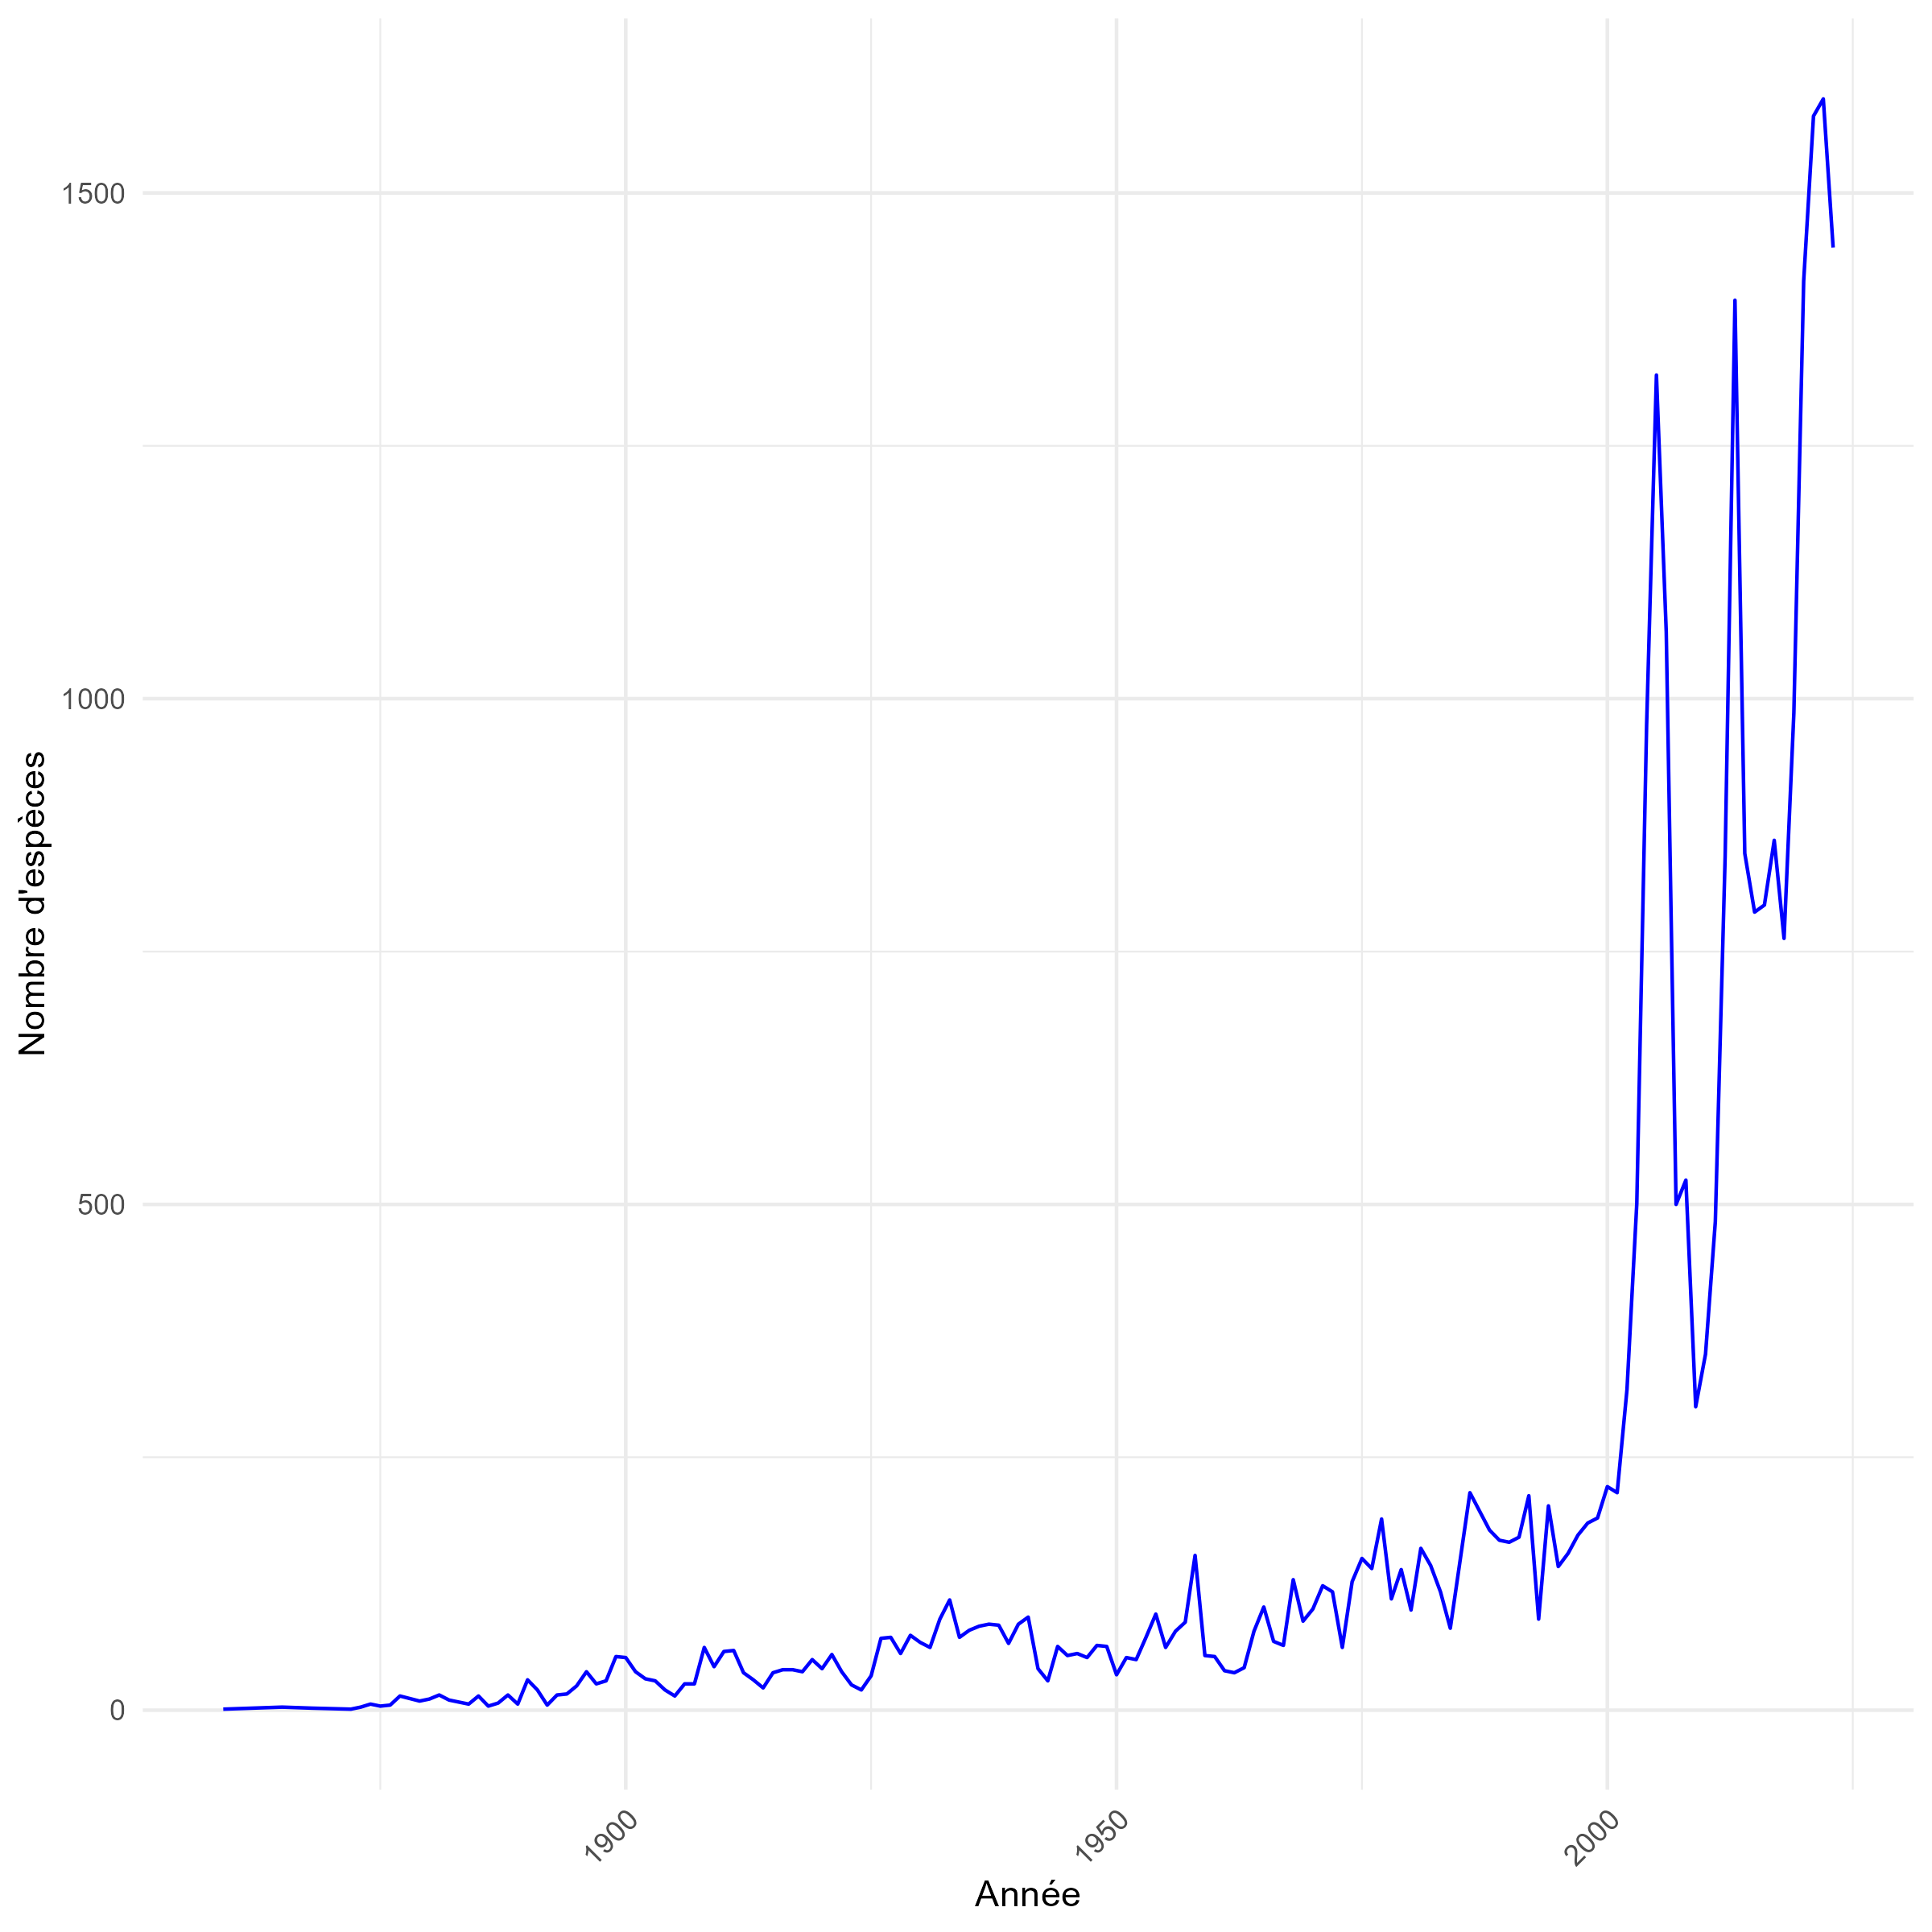
\includegraphics[keepaspectratio]{graphique_richesse.png}}

Dans la Figure 2, on remarque une augmentation du nombre d'espèces de
lépidoptères observées au fil des années. En effet, de 1860 à 1950, le
nombre d'espèces a peu varié, et celui-ci a commencé à augmenter entre
1950 et 2000. Une augmentation drastique peut être aperçue à partir des
années 2000, où le nombre d'espèces observées est passé d'environ 250
individus à plus de 1500. Cependant, entre les années 2000 et 2020, des
fluctuations peuvent être observées, où le nombre d'espèces diminue à
moins de 500 individus.

\begin{center}\rule{0.5\linewidth}{0.5pt}\end{center}

\begin{Shaded}
\begin{Highlighting}[]
\CommentTok{\#knitr::include\_graphics("./scripts/Rapport\_lepidopteres/graphique\_carte.png")}
\end{Highlighting}
\end{Shaded}

Dans la Figure 3, il est possible d'observer la distribution de la
richesse spécifique des lépidoptères au Québec en 2020. On remarque que
l'endroit où le nombre d'espèces est le plus élevé, soit près de 600,
est au nord-ouest de la province, près de 48°N et 80°W. Toutefois, des
richesses spécifiques d'environ 500 espèces sont retrouvées à l'ouest,
au sud et à l'est de la province. Il est également possible de remarquer
qu'il y a une plus forte concentration dans le sud de la province, près
du fleuve Saint-Laurent, que dans le nord de la province.

\vspace{10pt}

\textbf{Discussion }

Il est possible de confirmer un déplacement spatial modéré vers le nord
dans la distribution de certaines espèces de lépidoptères (Figure 1).
Selon Bernabé-Ruiz, Jiménez-Nieva, and Pérez-Quintero (2024),
l'augmentation des températures peut favoriser une migration vers des
latitudes plus élevées ainsi qu'une expansion des aires de répartition.
En effet, le déplacement de certaines espèces vers des répartitions plus
nordiques peut indiquer que les conditions environnementales y
deviennent plus favorables, en réponse au réchauffement des habitats
d'origine (Haris et al. 2024). Plusieurs facteurs peuvent expliquer
cette migration, notamment les variations plus extrêmes des
températures, l'irrégularité des précipitations entraînant des
sécheresses et des inondations, ainsi que la dégradation des habitats
(Haris et al. 2024). Cependant, différentes espèces de lépidoptères vont
réagir de manières différentes face aux changements climatiques en
fonction de leurs préférences alimentaires, de leurs exigences pour
l'habitat et de leur relation avec les plantes hôtes (Hussain et al.
2022). Puisque la température est un facteur limitant les aires de
répartition des plantes hôtes, ceci peut également limiter les aires de
distribution des lépidoptères, indépendamment de leur tolérance au
réchauffement climatique (White 2005). Selon Andrieux (2016), la
corrélation entre la température et la biodiversité pourrait entraîner
le déplacement des aires de répartition de plusieurs espèces au Québec,
ce qui pourrait expliquer en partie les tendances observées dans la
Figure 1.

Il est également possible de confirmer une augmentation du nombre
d'espèces de lépidoptères observées au fil des années (Figure 2). Bien
que cette augmentation puisse être influencée par des facteurs
écologiques, l'amélioration de l'effort d'échantillonnage est
probablement l'une des causes principales des résultats obtenus. En
effet, les données utilisées proviennent de base de données ouvertes,
compilant des observations de plusieurs individus. Puisqu'il y a eu une
augmentation significative de l'effort d'échantillonnage dans les
dernières années, il est normal que le nombre d'espèces ait augmenté
(Figure 2). Toutefois, les fluctuations observées entre les années 2000
et 2020 peuvent être expliquées par plusieurs facteurs, dont les
changements climatiques. Selon Haris et al. (2024), différents groupes
de pollinisateurs réagissent différemment, mais la majorité des familles
de lépidoptères a connu un déclin au cours des deux dernières décennies.
En effet, des études menées dans l'État de Ohio ont démontré qu'entre
1997 et 2017, la densité de 40\% des espèces de lépidoptères avait
diminué (Haris et al. 2024), ce qui concorde partiellement avec les
résultats obtenus dans la Figure 2.

Finalement, la Figure 3 démontre une forte richesse spécifique de
lépidoptères concentrée dans le sud du Québec, près du fleuve
Saint-Laurent. Cette distribution illustre l'influence des conditions
écologiques locales sur la densité de lépidoptères. En effet, selon
White (2005), la richesse spécifique des lépidoptères augmente dans les
pâturages, par rapport aux zones agricoles autour des cultures. De plus,
la fragmentation d'habitat semble être un facteur important pour la
distribution des lépidoptères, car la richesse spécifique des espèces
décroît lorsque la distance entre les habitats favorables augmente
(White 2005). Puisque les différentes espèces de lépidoptères ont
différentes préférences quant à leur habitat, une hétérogénéité élevée
des habitats favorise une richesse spécifique élevée (White 2005). Selon
Bernabé-Ruiz, Jiménez-Nieva, and Pérez-Quintero (2024), 80\% de la
variance de richesse spécifique peut être expliquée par les changements
climatiques, et ce phénomène est plus marqué dans les milieux ouverts,
notamment en raison de l'abandon de pâturage et de la fauche. De plus,
les lisières constituent des endroits privilégiés par les lépidoptères
grâce à leur abondance de ressources alimentaires, la température et
l'humidité (Ruchin 2023). Ces différents facteurs écologiques peuvent
expliquer la distribution concentrée de richesse spécifique de
lépidoptères au sud du Québec, mais un facteur non-négligeable est le
biais d'échantillonnage qui reflète le manque de données dans le nord de
la province.

\vspace{10pt}

\textbf{Conclusion}

En conclusion, la structure des communautés de lépidoptères au Québec
est affectée par des changements spatio-temporels. En effet, les aires
de répartition de certaines espèces sont influencées par le
réchauffement climatique et se déplacent vers le nord, ce qui permet de
confirmer la première hypothèse. Toutefois, bien que le nombre d'espèces
de lépidoptères observées semble augmenter au fil des années, des
diminutions importantes depuis les dernières décennies invalident
partiellement la deuxième hypothèse. La dernière hypothèse peut être
confirmée, car la distribution de la richesse spécifique des
lépidoptères au Québec est plus concentrée dans le sud de la province,
près des régions urbaines. Ces variations démontrent la sensibilité des
lépidoptères aux changements environnementaux et illustrent la réponse
de la biodiversité face aux pressions anthropiques. Pour limiter ces
impacts, il est essentiel de maintenir des milieux hétérogènes, de
limiter la fragmentation des habitats et de favoriser leur connectivité
(López-Vázquez et al. 2024). Par ailleurs, la mise en place de
protocoles de collecte de données et la réduction de biais
d'échantillonnage sont primordiales afin d'assurer un suivi à long terme
fiable de l'évolution des communautés face aux changements climatiques.

\section{Références}\label{ruxe9fuxe9rences}

\pnasbreak

\protect\phantomsection\label{refs}
\begin{CSLReferences}{1}{0}
\bibitem[\citeproctext]{ref-Andrieux2016}
Andrieux, B. 2016. {``Étude de La Migration Potentielle Des Niches
Écologiques Liées Aux Changements Climatiques Dans La Région Des Parcs
Nationaux de Frontenac Et Du Mont-Mégantic.''} Master's thesis,
Sherbrooke: Université de Sherbrooke.

\bibitem[\citeproctext]{ref-BernabeRuiz2024}
Bernabé-Ruiz, P. F. J., J. C. Jiménez-Nieva, and J. C. Pérez-Quintero.
2024. {``Temporal Variation and Influence of Environmental Variables on
a Lepidopteran Community in a Mediterranean Mid-Mountain Area.''}
\emph{Diversity} 16: 408. \url{https://doi.org/10.3390/d16070408}.

\bibitem[\citeproctext]{ref-Haris2024}
Haris, A., Z. Jozan, L. Roller, P. Sima, and S. Toth. 2024. {``Changes
in Population Densities and Species Richness of Pollinators in the
Carpathian Basin During the Last 50 Years (Hymenoptera, Dipetera,
Lepidoptera).''} \emph{Diversity} 16: 328.
\url{https://doi.org/10.3390/d16060328}.

\bibitem[\citeproctext]{ref-Hussain2022}
Hussain, Z. Z., Mahanood Sarwar, A. Akbar, S. K. Alhag, N. Ahmed, P.
Alam, A. A. Almadiy, F. Zouidi, and N. Barburao Jawalkar. 2022.
{``Spatiotemporal Distribution Patterns of Pest Species (Lepidoptera:
Noctuidae) Affected by Meteorological Factors in an Agroecosystem.''}
\emph{Agriculture} 12: 2003.
\url{https://doi.org/10.3390/agriculture12122003}.

\bibitem[\citeproctext]{ref-LopezVazquez2024}
López-Vázquez, K. L., P. Carlos, P. Corcuera, and C. Castillo-Guevara.
2024. {``Temporal Shifts in Flower-Visiting Butterfly Communities and
Their Floral Resources Along a Vegetation Type Altered by Anthropogenic
Factors.''} \emph{Forest} 15 (9): 1668.
\url{https://doi.org/10.3390/f15091668}.

\bibitem[\citeproctext]{ref-Ruchin2023}
Ruchin, A. B. 2023. {``Spatial Distribution of Lepidoptera in Forest
Ecosystems of Central European Russia: Studies Using Beer Traps.''}
\emph{Forests} 14: 680. \url{https://doi.org/10.3390/f14040680}.

\bibitem[\citeproctext]{ref-White2005}
White, P. J. 2005. {``Spatial and Temporal Patterns and Predictors of
Butterfly Species Richness in Canada Throughout the 20th Century.''}
Master's thesis, Ottawa: Université d'Ottawa.

\end{CSLReferences}



% Bibliography
% \bibliography{pnas-sample}

\end{document}
